\documentclass[aspectratio=169,28pt]{beamer}

\usepackage[utf8]{inputenc}
\usepackage[czech]{babel}
\usepackage{graphicx}
\usetheme{Madrid}
\usecolortheme{whale}
\usepackage[inline]{enumitem}
\usepackage{xcolor}

\beamertemplatenavigationsymbolsempty
\makeatletter
\defbeamertemplate*{footline}{Dan P theme}
{
  \leavevmode%
  \hbox{%
  \begin{beamercolorbox}[wd=.2\paperwidth,ht=2.25ex,dp=1ex,center]{author in head/foot}%
    \usebeamerfont{author in head/foot}\insertshortauthor\expandafter\beamer@ifempty\expandafter{\beamer@shortinstitute}{}{~~(\insertshortinstitute)}
  \end{beamercolorbox}%
  \begin{beamercolorbox}[wd=.6\paperwidth,ht=2.25ex,dp=1ex,center]{title in head/foot}%
    \usebeamerfont{title in head/foot}\insertshorttitle
  \end{beamercolorbox}%
  \begin{beamercolorbox}[wd=.2\paperwidth,ht=2.25ex,dp=1ex,right]{date in head/foot}%
    \usebeamerfont{date in head/foot}\insertshortdate{}\hspace*{2em}
\insertframenumber{} / \inserttotalframenumber\hspace*{2ex} 
  \end{beamercolorbox}}%
  \vskip0pt%
}
\makeatother


\title{Evaluace algoritmů\\ lokálně senzitivního hashování (LSH)\\ v doporučovacích systémech}
\author{Ladislav Martínek}

\begin{document}

\section{Úvod}
\begin{frame}
\titlepage
\end{frame}

\section{Cíle BP}
\begin{frame}{Cíle Bakalářské práce}
       \begin{itemize}
		\item[•] Analýza metod LSH 
		\item[•] Návrh aplikace metod do algoritmu k-NN 
		\item[•] Návrh a implementace testovací knihovny
		\item[•] Testování různých parametrizací LSH
		\item[•] Diskuze výsledků
		\end{itemize}
\end{frame}

\section{Motivace}
\begin{frame}{Motivace}
		\begin{itemize}
		\item[•] Osobní zájem v oblasti doporučovacích systémů
		\item[•] Narůstajícího množství dat
		\item[•] Osobní přínos
		\end{itemize}
\end{frame}

\section{Odborné pojmy}
\begin{frame}{Specifikace problematiky}
		\begin{itemize}
		\item[•] Kolaborativní filtrování
		\item[•] User-based k-NN
		\item[•] Kosinova podobnost
		\item[•] Lokálně senzitivní hashování
		\end{itemize}
\end{frame}



\section{Návrh systému}
\begin{frame}{Návrh}
\begin{columns}[c]
    \column{7cm}
      \begin{itemize}
		\item[•] Předzpracování
		\item[•] Modul k-NN
		\item[•] Modul LSH
		\item[•] Testování přesnosti k-NN a úspěšnosti doporučování 
		\end{itemize}
    \column{8cm}
      \center\includegraphics[width=7cm]{img/schemaBP}
  \end{columns}
		
\end{frame}

\section{Metody LSH a hashovací funkce}
\begin{frame}{Metody LSH a hashovací funkce}
		\begin{itemize}
		\item[•] Projekční matice
		\item[•] Počet hashovacích funkcí
		\item[•] Multi-probe
		\item[•] Popularita položek  
		\end{itemize}
\end{frame}

\section{Implementace}
\begin{frame}{Realizace}
		\begin{itemize}
		\item[•] Python
		\item[•] Modul pro tvorbu grafů
		\item[•] Argumenty
		       \begin{description}
		       \item[\textbf{-d}] Dimenze hashovací funkce
		       \item[\textbf{-c}] Nastavení metody multi-probe
		       \item[\textbf{-m}] Hashovací funkce
		       \item[\textbf{-M}] Standartní hashovací funkce
		       \end{description}
		\end{itemize}
\end{frame}

\section{Princip testování}
\begin{frame}{Princip testování}
		\begin{itemize}
		\item[•] Testování na přesnost 10-NN
		\item[•] Úspěšnost doporučování na vybraných modelech 
		\item[•] Databáze A
		       \begin{description}
		       \item[\textbf{záznamu uživatel-položka:}] 1 280 189
		       \item[\textbf{uživatelů:}] 290 625
		       \item[\textbf{položek:}] 11 101
		       \end{description}
		\item[•] Databáze B
		       \begin{description}
		       \item[\textbf{záznamu uživatel-položka:}] 54 234 951
		       \item[\textbf{uživatelů:}] 1 028 287
		       \item[\textbf{položek:}] 52 689
		       \end{description}
		\end{itemize}
\end{frame}

\section{Výsledky testování}
\begin{frame}{Výsledky testování}
\begin{columns}[c]
    \column{7cm}
      \begin{itemize}
		\item[•] Přesnost 10-NN
		\item[•] Úspěšnost doporučování (recall a~catalog coverage)
		\item[•] Závislost přesnosti 10-NN a hodnoty recall
		\end{itemize}
    \column{8cm}
      \center\center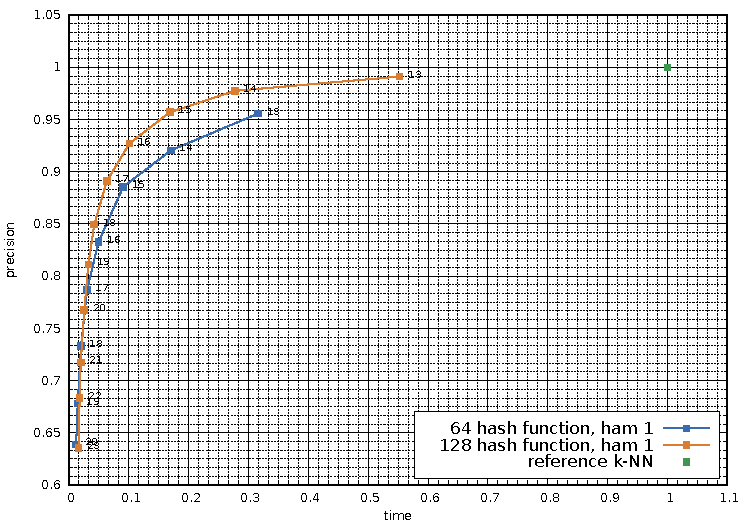
\includegraphics[width=8cm]{img/modKNNopt}
  \end{columns}
		
\end{frame}

\section{Závěr}
\begin{frame}{Závěr}
		\begin{itemize}
		\item[•] Dosažené výsledky
		\item[•] Nastavení modelů
		\item[•] Budoucí práce
		\end{itemize}
\end{frame}

\section{Použitá literatura}

\begin{frame}{Použité literární zdroje}
		\begin{thebibliography}{9}
\small

\bibitem{handbook}
  \color{black}RICCI, F.; ROKACH, L.; SHAPIRA, B.; aj.: \textit{Recommender systems handbook.} Springer New York Dordrecht Heidelberg London, 2011, ISBN 978-0-387-85819-7.
  
  \bibitem{collaborative}
  \color{black}XUE, G.-R.; LIN, C.; YANG, Q.; aj.: Scalable collaborative filtering using cluster-based smoothing. [online], August 15 - 19, 2005, [cit. 2018-03-08]. Dostupné z: \url{https://dl.acm.org/citation.cfm?id=1076056}
  
  \bibitem{survey}
  \color{black}WANG, J.; SHEN, H. T.; SONG, J.; aj.: Hashing for Similarity Search: A Survey. [online], Submitted on 13 Aug 2014, [cit. 2018-03-11], 1408.2927. Dostupné z: \url{http://arxiv.org/abs/1408.2927}
  
  \bibitem{multiprobe}
  \color{black}LV, Q.; JOSEPHSON, W.; WANG, Z.; aj.: Multi-probe LSH: efficient indexing for high-
dimensional similarity search. [online], September 23 - 27, 2007, [cit. 2018-03-17]. Dostupné z: \url{http://dl.acm.org/citation.cfm?id=1325851.1325958}

  \bibitem{popularity}
  \color{black}STECK, H.: Item Popularity and Recommendation Accuracy. [online], October 23 - 27, 2011, [cit. 2018-03-19]. Dostupné z: \url{doi:10.1145/2043932.2043957}

\end{thebibliography}
		
\end{frame}

\section{Poděkování}

\begin{frame}
		\Huge\center{Děkuji za pozornost!}
		\vskip 15pt
		{\color{blue}\rule[2pt]{0.8\textwidth}{2pt}}
		\color{black}\vskip 15pt
		\LARGE\center{Dotazy?}
\end{frame}


\end{document}

